\chapter{Paradigm Shift}
Il Paradigm Shift rappresenta una importante caratteristica di tutti i fenomeni sociali ma principalmente economici che evidenzia un completo cambiamento di direzione, qualcosa che rompe gli equilibri e rende evidenti nuovi bisogni che possono essere soddisfatti con nuove soluzioni e tecnologie. 

Cercare di capire quali tecnologie possono modificare il futuro in maniera significativa a medio e breve termine ci permette di investire su quelle tecnologie. Vedremo nel dettaglio tre tipi di Paradigm Shift (Social, Work, Business).

\section{Paradigm Shift e Disruptive Technology}
Una delle maggiori aziende di consulenza direzionale che si occupa di effettuare analisi di mercato, Gartner, ha sviluppato uno strumento chiamato \textbf{Hype Cycle}. Il punto fondamentale è distinguere le promesse di ambizione e successo e di nuovi servizi da quella che è l'esagerazione (hype), che rende le cose presentate più belle e importanti di quello che siano. Bisogna capire quindi quando queste tecnologie riescono finalmente a ripagare degli investimenti. 

\noindent L'Hype Cycle è uno strumento usato con molta diffusione per descrivere questi fenomeni e quindi è perfetto per rappresentare il livello di maturità, di adozione e applicazione di una certa tecnologia. 

\begin{figure}[ht]
    \centering
    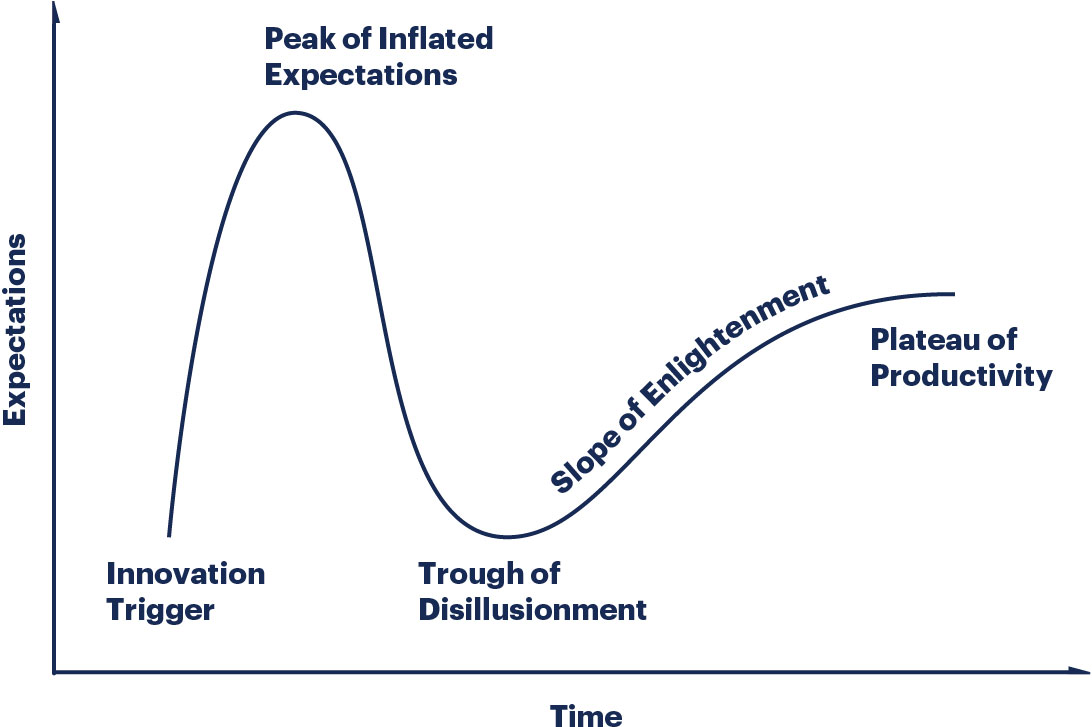
\includegraphics[width=8cm]{./Images/cap4/4.1.jpg}
\end{figure}

\noindent La dinamicità offerta da questo strumento permette alle tecnologie di muoversi sulla curva a velocità differenti. Distinguamo le diverse fasi:
\begin{itemize}
    \item \textbf{Innovation Trigger}: nasce una nuova tecnologia che rappresenta qualcosa di molto innovativo, e viene immediatamente recepita e catturata dai media e iniziano ad apparire delle prime \textit{proof of concept}. A questo punto però affidabilità e commercializzabilità sono ancora da scoprire: a volte può capitare che certe tecnologie abbiano bisogno di competenze specifiche o di vincoli stretti sulle infrastrutture interne, e quindi soffrire di una bassa commercializzabilità.
    \item \textbf{Peak of Inflated Expectations}: il momento della vetta delle attese gonfiate è quando la pubblicità continua a produrre \textit{success stories}, mentre ai fallimenti che vengono identificati non si dà altrettanto peso. Una volta arrivati in cima al picco, si cade nell'abisso della disillusione.
    \item \textbf{Trough of Disillusionment}: appena la tecnologia supera il picco, vengono immediatamente enfatizzati i fallimenti che prima erano stati messi da parte e iniziano ad esserci i problemi dei produttori, che possono potenzialmente fallire. I provider che sopravvivono cercano di migliorare il prodotto per risollevarsi e convincersi che sia una buona tecnologia. Questi spesso vengono chiamati \textit{early adopters}.
    \item \textbf{Slope of Enlightenment}: si iniziano ad evidenziare i benefici della tecnologia che vengono dimostrati all'interno delle aziende perché iniziano ad apparire la seconda e la terza generazione, e se la disillusione non è stata sufficiente a buttare via i produttori dal mercato, alla fine si riesce ad arrivare al pianoro della produttività.
    \item \textbf{Plateau of Productivity}: finalmente le principali aziende adottano la tecnologia ed iniziano a comparire dei criteri per definire l'affidabilità dei provider in modo da creare un mercato in cui il valore appare chiaro. I brand principali iniziano ad avere i vantaggi da questo punto di vista.
\end{itemize}
\subsection{Le rivoluzioni nel Paradigm Shift}
Le rivoluzioni tecnologiche avvengono quando viene avvertita la possibilità di cambiare in maniera radicale le nostre abitudini con cui approcciamo ad un sistema. Il progresso non è stabile, ci sono miglioramenti che portano a queste modifiche: vengono rotti degli equilibri e mostrano nuovi scenari di business. Il ruolo della \textbf{disruptive technology} può essere notato facilmente nel grafico seguente.

\begin{figure}[ht]
    \centering
    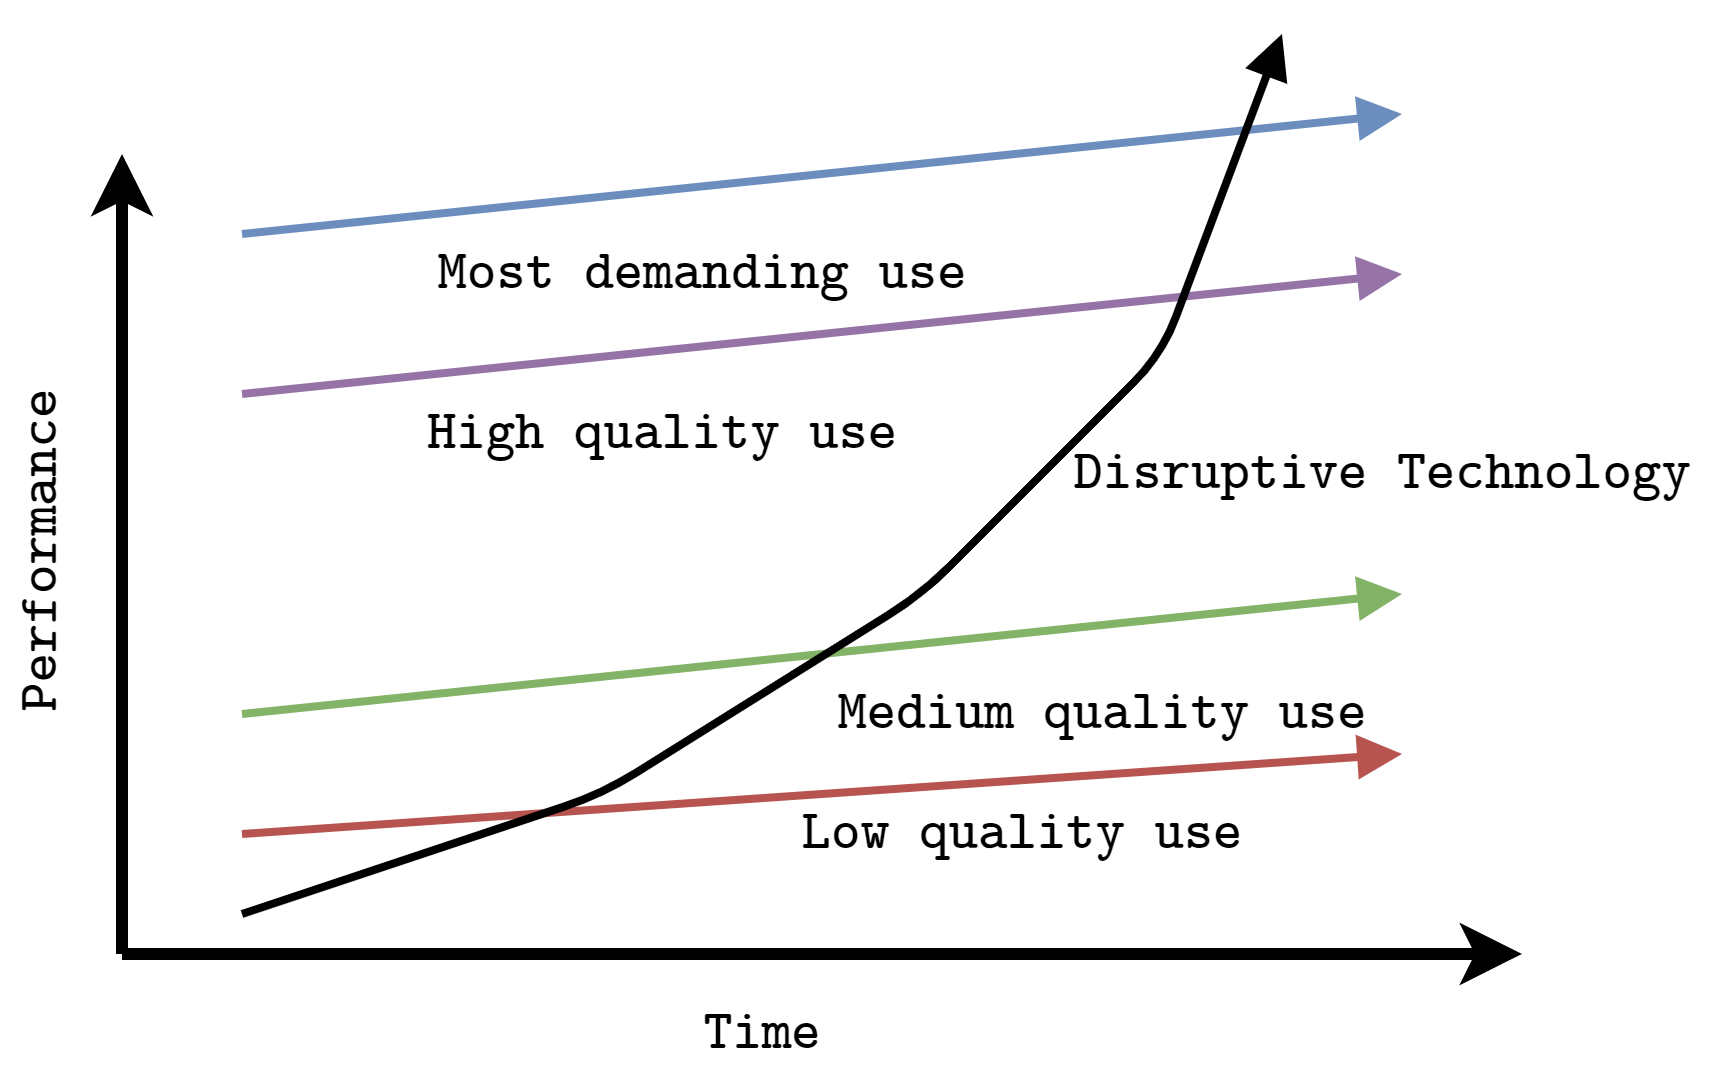
\includegraphics[width=8cm]{./Images/cap4/4.2.png}
\end{figure}

Una tecnologia di basso livello è in grado di assicurare un miglioramento di prestazioni nel tempo. La disruptive technology invece riesce ad assicurare molto velocemente il cambiamento e la qualità di prestazioni sul tempo e chiaramente riesce a soppiantare queste tecnologie perché assicura un altissimo payoff in pochissimo tempo. Alcune disruptive technologies:
\begin{itemize}
    \item Automobili: quando Henry Ford chiese ai suoi clienti cosa volessero, questi risposero cavalli più veloci e più resistenti;
    \item Fotocamere digitali: hanno portato alla chiusura di fabbriche di rullini fotografici, brand e reti di distribuzione;
    \item Musicassette, dischi in vinile, CD.
\end{itemize}
\subsection{Scientific Paradigm Shift}
Possiamo distinguere alcuni dei paradigmi utilizzati nella computer science. La prima azienda fu IBM con l'invenzione del Personal Computer, in pratica ogni utente poteva possedere una macchina.  Microsoft invece asserì la commerciabilità del sofware, ovvero di qualcosa di intangibile rispetto all'hardware: era importante costruire computer ma era importante scrivere software innovativo e piazzarlo su ogni computer per creare un mercato (che poi è diventato quasi un monopolio). DELL invece fu la prima azienda a permettere la possibilità di acquistare computer secondo delle configurazioni hardware personalizzate.

\section{Social Paradigm Shift}
Il cloud influenza la vita sociale delle persone in maniera significativa, in un certo senso può essere considerato come un agente di cambiamento. Quando parliamo di Social Paradigm Shift ci vengono subito in mentre tre applicazioni: societal cloud, personal cloud e cloud of things.

\subsection{Societal Cloud}
Un Societal Cloud è un tipo di cloud che serve una community. In questo ambito l'utilizzo di modelli PaaS fornisce una serie di servizi che permette alle community di lavorare, offrendo un ambiente sicuro che ha una sua contestualizzazione a livello internazionale e nazionale (EU e NATO sono societal clouds). Una community cloud si occupa di convertire i social media a cloud sociali usando le caratteristiche del cloud: dal punto di vista individuale potrebbe non essere considerato un paradigm shift in quanto già tutti utilizziamo i social. Tuttavia dal punto di vista della community è più semplice riuscire a definire dei servizi che vengono personalizzati in base alle necessità delle community.

\subsection{Personal Cloud}
Ogni giorno utilizziamo il Personal Cloud (esempi sono Dropbox o Google Drive), sia per svago e divertimento oppure per finanza e shopping. Sono elementi importanti, infatti man mano che i servizi diventano economici (e a volte gratuiti) diventa più semplice avere un proprio spazio online come strumento di comunicazione (YouTube, Twitch).
\subsection{Cloud of Things}
Come l'Internet of Things riguarda tutto ciò che comprende la domotica e la gestione della sicurezza. Può essere integrato nell'ambiente di lavoro con diverse possibilità, le quali possono essere realizzate con l'automazione di determinate task.

\section{Work Paradigm Shift}
Riguarda due importanti trend abilitati dal cloud:
\begin{itemize}
    \item Rimpiazzare le workstation con \textit{thin client}, che non possono compiere operazioni se non quelle abilitate dal cloud: la gestione di un laptop prende tempo (c'è bisogno di manutenzione continua per sofware, sistema operativo). L'idea è quella di accedere a terminali da remoto: il lavoro di gestione delle macchine è semplificato perche si trovano fisicamente tutti insieme. Il secondo beneficio è che i dati si trovano sul cloud, quindi la macchina è indipendente e non pone alcun problema per la sicurezza.
    \item Ubiquitous computing: seguendo il paradigma del \textit{Bring Your Own Device} (BYOD), l'idea è quella di poter utilizzare qualsiasi periferica per lavorare. In questo modo l'IT department assume sempre più il ruolo di Cloud Service Broker. Tutto ciò è possibile grazie a dei meccanismi di sandbox presenti sulle macchine che permettono di memorizzare dati critici e criptare i dati nel caso in cui la periferica cada in mani sbagliate.
\end{itemize}

\section{Business Paradigm Shift}
Dal punto di vista del business c'è un aspetto particolarmente importante che va considerato: nelle grandi aziende c'è una relazione tra Work Paradigm Shift e Business Paradigm Shift: il primo punto imporante è quello del dipartimento IT, che possiamo immaginare come la divisione di un'azienda che fornisce supporto IT per l'azienda stessa (ovviamente nel caso in cui il core business non riguardi l'IT). Il punto cruciale è che spesso c'è uno scollamento tra la gestione dell'IT fatta dal dipartimento e quella legata al business, che spesso è gestita localmente dalla business unit. 

Il Business Paradigm Shift è motivato da ragioni immediate a breve termine di efficienza: una macchina la cui configurazione è gestita dal suo diretto utilizzatore è pronta in modo più veloce.

\vspace{5mm}

Quello che tipicamente si fa è utilizzare il modello \textit{hub and spoke}, nel quale i servizi centralizzati fungono da hub (mail, servizi di rete, periferiche di stampa, gruppi di continuità) e i gruppi di business lavorano autonomamente, ovvero dalle proprie macchine e gestite in maniera separata. Questo fenomeno è anche conosciuto come \textbf{Shadow IT} e riguarda le applicazioni di cui il dipartimento centrale IT non è consapevole né responsabile. Di solito se capita un problema il supporto è molto complesso.

Un central IT department molto forte dovrebbe rifiutarsi di offrire supporto per shadow IT, in quanto questo è un rischio per il business.

\section{Learning Check}
\begin{enumerate}
    \item Quali sono i \textit{social paradigm shift} indotti dal cloud computing?
    \item Come è cambiata (e cambierà) l'esperienza lavorativa a causa del cloud computing?
    \item Qual è il \textit{business paradigm shift} più comune?
\end{enumerate}
